
\documentclass {article}
\usepackage{graphicx}
\usepackage[hypcap]{caption}
\usepackage{amssymb,amsmath}
\begin{document}
\title{CSE603 Assignment3}
\author {Ruhan Sa 50060400}
\maketitle
\noindent \textbf{Aim}: Compute the product of matrix A and matrix B. Result stored into C using Netezza.

\noindent \textbf{Verification}:  This is done using matrix with unit elements and the result is verified by checking wether elements of C equals to the matrix size or not. If so the implementation is verified, if not the implementation is wrong.

\noindent \textbf{Script}: All the compilations and SQL scripts that may have used is attached in source code as comment.

\section{Source code explanation}
\subsection{Input function}
Both A and B are generated using UDTF functions Ain(int, int) and Bin(int, int), where matrix size and input routines ( 0 or 1) are taken as first and second input parameters respectively. 0 indicates the verification input routine, where the elements are chosen as unity, and 1 indicates the computational experimental input routine, where the matrix element is chosen as random numbers ranges from 0 to 2. SPU distribution on row numbers and column numbers are used for A and B to speed up the result. 
\begin{figure}[htp!]
\centering
\includegraphics[width = \linewidth]{1.pdf}
\caption{Table layout}
\label{fig:one}
\end{figure}
Figure 1 shows the table layout of A and B.

\subsection{Output function}
The time taken to do multiplication is done using SQL command line -- time. 
The multiplication of the matrix is done by UDTF function rout(int, int, varchar, varchar), where first two parameters denote the row and column number, last two parameter denote the row and column element needed from A and B. The element of A and B are passed into UDTF function parameters.

\section {Experimental result}
\subsection{Time consumption with the increase of matrix size}
Figure 2 shows the time consumption of NETEZZA with the increase of matrix size. The time consumption is computed as the sum of matrix input time and matrix output time. Matrix input time indicates the time of creating matrix A, B and the time for creating Tables for each of the matrix in database. Matrix output time indicates the time taken to do matrix multiplication and create table C to store the result into database. 

\begin{figure}[htp!]
\centering
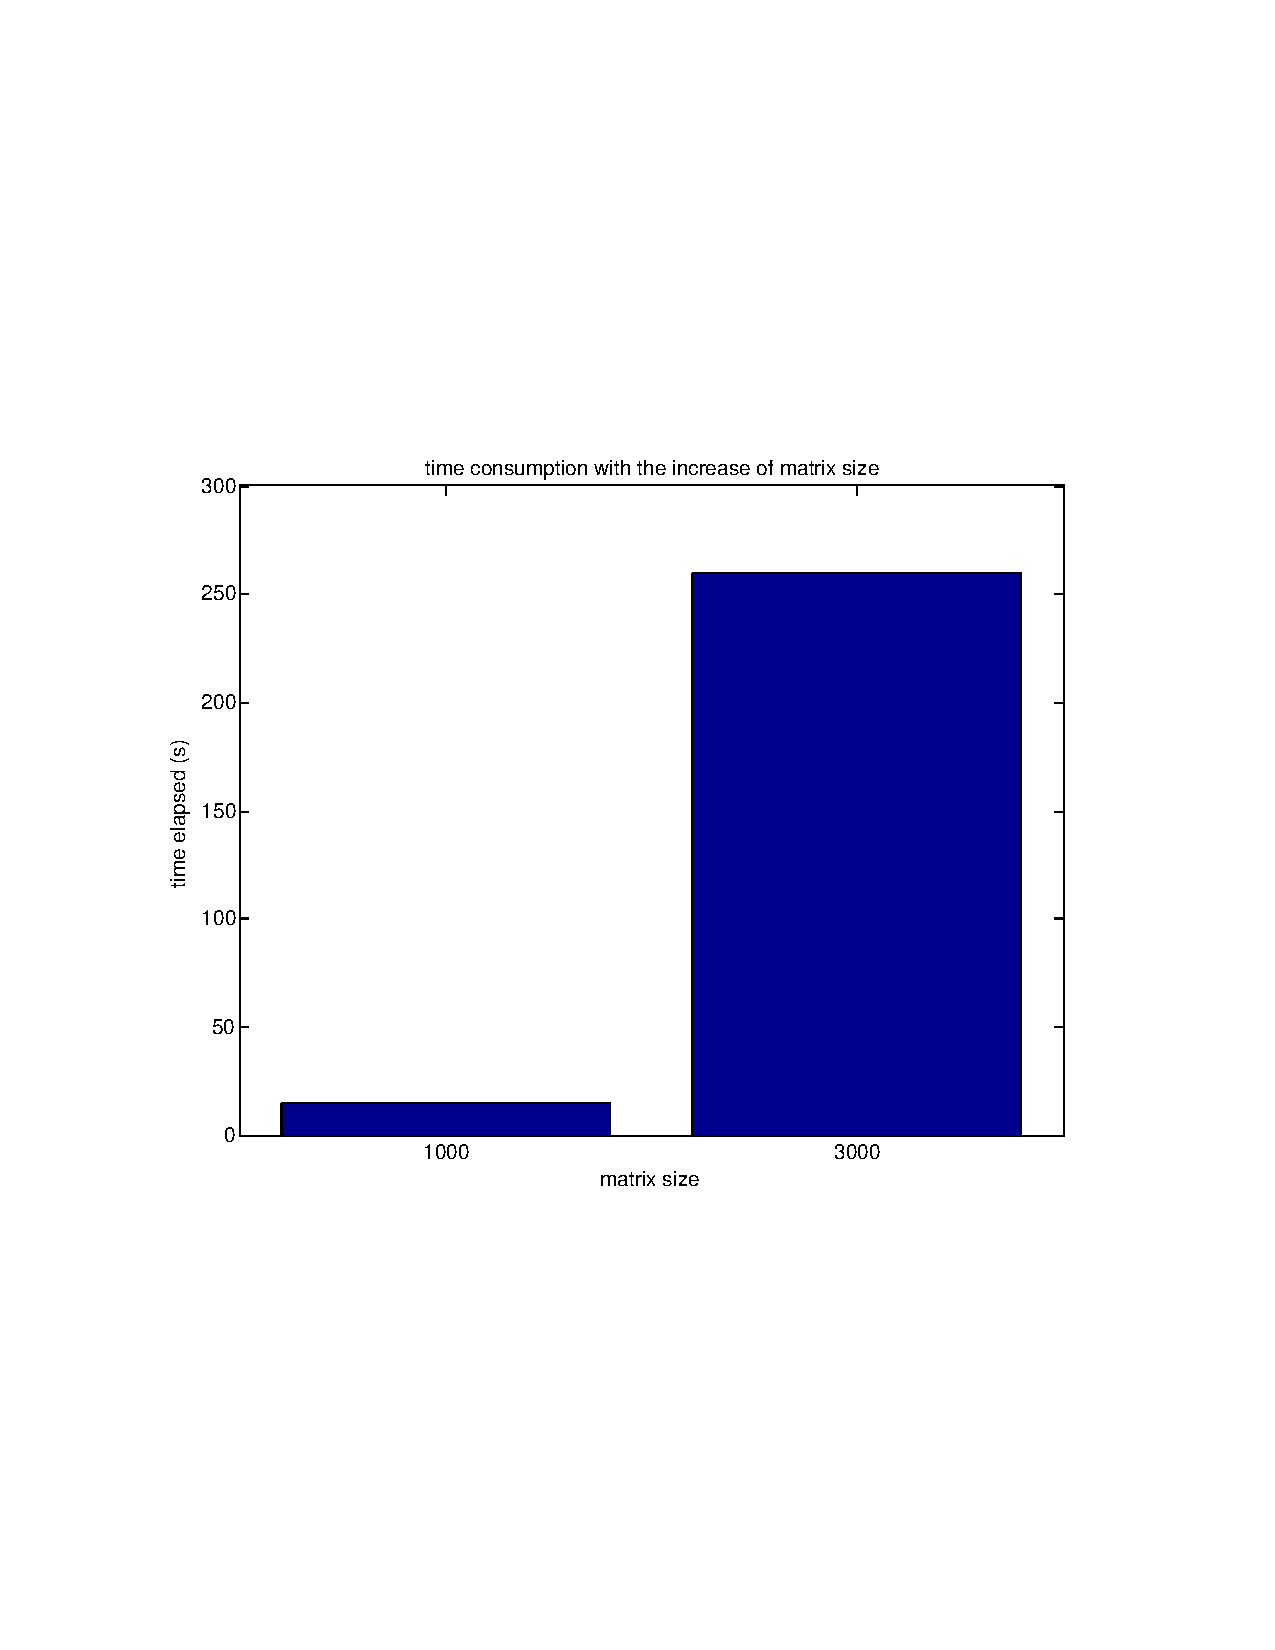
\includegraphics[width = \linewidth]{2.pdf}
\caption{Time consumption with two different matrix size.}
\label{fig:two}
\end{figure}

\begin{figure}[hbp!]
\centering
\includegraphics[width = \linewidth]{3.pdf}
\caption{Time consumption comparison with MPI, OMP and GPU.}
\label{fig:one}
\end{figure}



\subsection{Comparison with MPI, OpenMP and GPU}
Figure 3 shows the performance comparison with OpenMP, MPI and GPU when computing matrix size of $1000 \times 1000$. Here the MPI performance was observed when using 20 processors, OpenMP performance was observed using 20 processors, the $gpu$ bar indicates the best performance chosen from last assignment. 

\end {document}
